\documentclass[tikz,border=10pt]{standalone}
\usepackage{amsmath,amssymb}
\usepackage{tikz}
\usetikzlibrary{arrows.meta,calc,angles,quotes,positioning}

\definecolor{navy}{HTML}{1B365D}
\definecolor{crimson}{HTML}{C0392B}
\definecolor{steelblue}{HTML}{2471A3}
\definecolor{teal}{HTML}{0E6251}
\definecolor{amber}{HTML}{D35400}
\definecolor{slate}{HTML}{566573}

\begin{document}
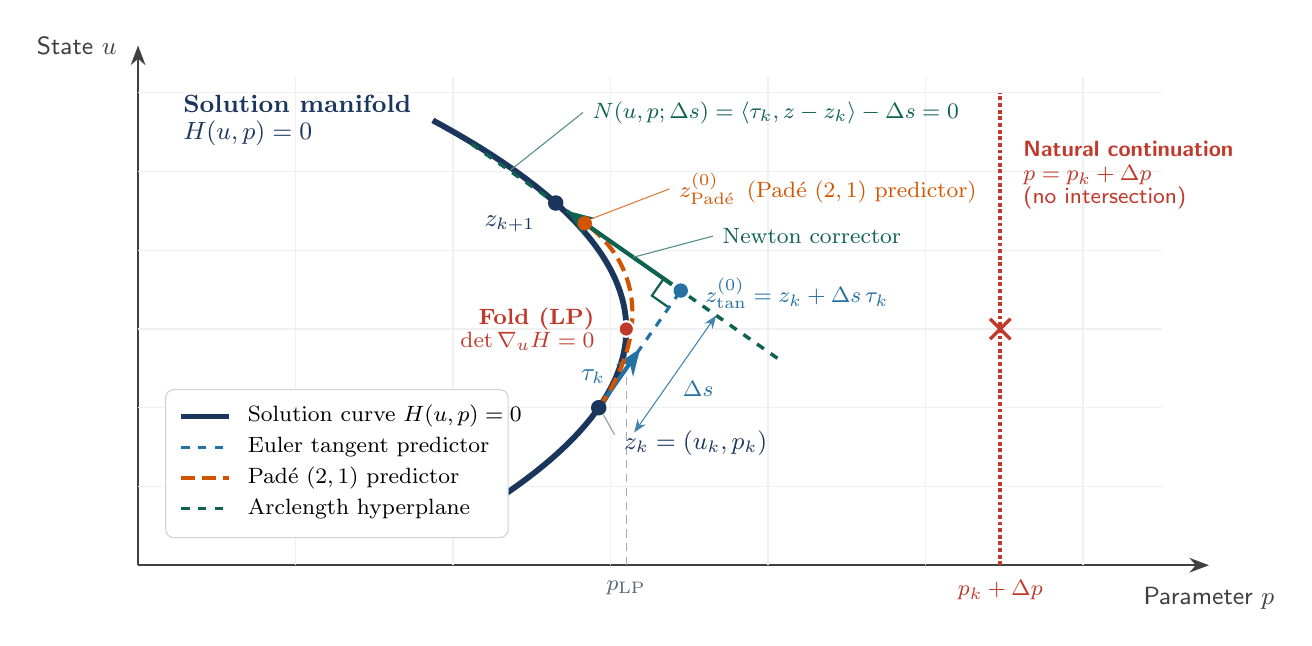
\begin{tikzpicture}[
    >=Stealth,
    font=\sffamily\small,
    axis/.style={->, thick, color=black!75, line width=0.9pt},
    manifold/.style={color=navy, line width=2.1pt},
    tangent/.style={->, color=steelblue, line width=1.5pt},
    predline/.style={dashed, color=steelblue, line width=1.15pt},
    hyperplane/.style={dashed, color=teal, line width=1.25pt},
    natural/.style={densely dotted, color=crimson, line width=1.4pt},
    pade/.style={color=amber, line width=1.5pt, dash pattern=on 5pt off 2.5pt},
    newton/.style={->, color=teal, line width=1.5pt},
    leader/.style={thin, color=black!40},
]

% Axes
\draw[axis] (0,0) -- (13.6,0) node[below=4pt] {Parameter $p$};
\draw[axis] (0,0) -- (0,6.6) node[left=4pt] {State $u$};

% Subtle grid
\foreach \y in {1,2,3,4,5,6} {\draw[black!6, thin] (0,\y) -- (13.0,\y);}
\foreach \x in {2,4,6,8,10,12} {\draw[black!6, thin] (\x,0) -- (\x,6.2);}

% Natural parameter continuation failure slice p = p_k + Delta p (well right of all labels)
\draw[natural] (10.95, 0) -- (10.95, 6.0);
\node[crimson, align=left, anchor=west, font=\sffamily\footnotesize] at (11.12, 4.95) {%
    \textbf{Natural continuation}\\[-1pt]
    $p = p_k + \Delta p$\\[-1pt]
    (no intersection)%
};
\draw[crimson, very thick] (10.82, 3.0 - 0.13) -- (11.08, 3.0 + 0.13);
\draw[crimson, very thick] (10.82, 3.0 + 0.13) -- (11.08, 3.0 - 0.13);
\node[crimson, font=\footnotesize, below=2pt] at (10.95, 0) {$p_k + \Delta p$};

% Fold vertical tangent reference (p_LP = 6.2)
\draw[slate!55, densely dashed, thin] (6.20, 0) -- (6.20, 3.0);
\node[slate, font=\footnotesize, below=2pt] at (6.20, 0) {$p_{\text{LP}}$};

% Solution manifold H(u,p) = 0: p(t) = 6.2 - 0.45*(t - 3.0)^2, u(t) = t
% At t = 1.75: p = 6.2 - 0.45*(1.25)^2 = 5.497, u = 1.75
%   dp/dt = 0.90*1.25 = 1.125, du/dt = 1.0 => norm = 1.5052 => tau = (0.7474, 0.6644)
% At t = 4.45: p = 6.2 - 0.45*(1.45)^2 = 5.254, u = 4.45
%   ds = (5.254 - 5.497)*0.7474 + (4.45 - 1.75)*0.6644 = -0.1816 + 1.7939 = 1.6123
% Wait: let's use t_k = 1.85, t_next = 4.55 so z_tan is well separated from fold:
%   t_k = 1.85 => p = 6.2 - 0.45*(1.15)^2 = 5.605, u = 1.85
%   dp/dt = 1.035, du/dt = 1.0 => norm = 1.4392 => tau = (0.7192, 0.6948)
%   normal = (-0.6948, 0.7192)
%   t_next = 4.55 => p = 6.2 - 0.45*(1.55)^2 = 5.119, u = 4.55
%   ds = (5.119 - 5.605)*0.7192 + (4.55 - 1.85)*0.6948 = -0.3495 + 1.8760 = 1.5265
%   z_tan = (5.605 + 1.5265*0.7192, 1.85 + 1.5265*0.6948) = (6.703, 2.911)
% Let's use gentler curve p(t) = 6.4 - 0.42*(t - 3.0)^2, t_k = 1.70, t_next = 4.60:
%   t_k = 1.70 => p = 6.4 - 0.42*1.69 = 5.690, u = 1.70
%   dp/dt = 0.84*1.30 = 1.092, du/dt = 1.0 => norm = 1.4807 => tau = (0.7375, 0.6754)
%   normal = (-0.6754, 0.7375)
%   t_next = 4.60 => p = 6.4 - 0.42*2.56 = 5.325, u = 4.60
%   ds = (5.325 - 5.690)*0.7375 + (4.60 - 1.70)*0.6754 = -0.2692 + 1.9587 = 1.6895
%   z_tan = (5.690 + 1.6895*0.7375, 1.70 + 1.6895*0.6754) = (6.936, 2.841)
%   Wait: z_tan at u = 2.841 is too close to fold u = 3.0.
%   To put z_tan nicely ABOVE the fold, take t_k closer to fold or larger ds:
%   Try p(t) = 6.2 - 0.40*(t - 2.8)^2, t_k = 1.60, t_next = 4.50:
%   Wait: let's just pick t_k = 2.00, t_next = 4.60 with p(t) = 6.2 - 0.35*(t - 3.0)^2:
%   t_k = 2.00 => p = 6.2 - 0.35 = 5.850, u = 2.00
%   dp/dt = 0.70, du/dt = 1.0 => norm = 1.2207 => tau = (0.5735, 0.8192)
%   normal = (-0.8192, 0.5735)
%   t_next = 4.60 => p = 6.2 - 0.35*(2.56) = 5.304, u = 4.60
%   ds = (5.304 - 5.850)*0.5735 + (4.60 - 2.00)*0.8192 = -0.3131 + 2.1299 = 1.8168
%   z_tan = (5.850 + 1.8168*0.5735, 2.00 + 1.8168*0.8192) = (6.892, 3.488)
%   dist(z_tan, z_next) = sqrt((6.892-5.304)^2 + (3.488-4.600)^2) = sqrt(2.522 + 1.237) = 1.939!
%   HUGE, clean separation! z_tan = (6.892, 3.488) is well above & right of fold (6.2, 3.0)!
%   z_pade = z_next - 0.45*normal = (5.304 + 0.45*0.8192, 4.600 - 0.45*0.5735) = (5.673, 4.342)
\draw[manifold, domain=0.60:5.65, samples=120, smooth]
    plot ({6.2 - 0.35*(\x - 3.0)*(\x - 3.0)}, {\x});

% Manifold label in open upper-left space
\node[navy, font=\bfseries\small, align=left, anchor=west] at (0.45, 5.65) {Solution manifold\\[-1pt]$H(u,p) = 0$};

% Exact coordinates
\coordinate (zk)     at (5.850, 2.000);
\coordinate (fold)   at (6.200, 3.000);
\coordinate (ztan)   at (6.892, 3.488);
\coordinate (znext)  at (5.304, 4.600);
\coordinate (zpade)  at (5.673, 4.342);
\coordinate (hp1)    at (8.120, 2.628);
\coordinate (hp2)    at (4.157, 5.403);
\coordinate (tauend) at ($(zk) + 0.92*(0.5735, 0.8192)$);

% Orthogonal hyperplane N(u, p; ds) = 0
\draw[hyperplane] (hp1) -- (hp2);

% Hyperplane equation placed cleanly above-right of hp2 (clear of all curves & red line!)
\node[teal, font=\footnotesize, anchor=west] (hplab) at (5.65, 5.75)
    {$N(u,p;\Delta s) = \langle \tau_k, z - z_k \rangle - \Delta s = 0$};
\draw[leader, teal!70] (hplab.west) -- (4.72, 5.01);

% Right-angle marker at z_tan
\pic[draw=teal, thick, angle radius=7.5pt] {right angle = zk--ztan--znext};

% Euler tangent predictor dashed line & unit tangent arrow
\draw[predline] (zk) -- (ztan);
\draw[tangent] (zk) -- (tauend);
\node[steelblue, font=\small, left=2pt] at ($(zk)!0.52!(tauend)$) {$\tau_k$};

% Step size ds dimension arrow offset cleanly to the right
\draw[<->, steelblue!85, thin]
    ($(zk) + (0.45, -0.315)$) -- ($(ztan) + (0.45, -0.315)$)
    node[midway, below right=-1pt, font=\footnotesize, steelblue] {$\Delta s$};

% Padé (2,1) curved predictor from z_k tangent to tau_k landing at z_pade on hyperplane
\draw[pade] (zk) .. controls (6.52, 2.96) and (6.36, 3.86) .. (zpade);

% Newton corrector projection arrow along hyperplane from z_tan -> z_next (slightly offset for clarity)
\draw[newton] ($(ztan) + (-0.11, 0.077)$) -- ($(znext) + (0.14, -0.098)$);
\node[teal, font=\footnotesize, anchor=west] (newtlab) at (7.30, 4.18) {Newton corrector};
\draw[leader, teal!70] (newtlab.west) -- ($(ztan)!0.38!(znext)$);

% Padé predictor label cleanly placed above-right with short leader
\node[amber, font=\footnotesize, anchor=west] (padelab) at (6.75, 4.78)
    {$z_{\text{Pad\'e}}^{(0)}$ \,(Pad\'e $(2,1)$ predictor)};
\draw[leader, amber!75] (padelab.west) -- ($(zpade) + (0.09, 0.06)$);

% Fold point marker & label in clear space to the left
\fill[crimson] (fold) circle (2.8pt);
\draw[white, thick] (fold) circle (2.8pt);
\fill[crimson] (fold) circle (2.2pt);
\node[crimson, font=\footnotesize, align=right, anchor=east] at (5.92, 3.00)
    {\textbf{Fold (LP)}\\[-1pt]$\det \nabla_u H = 0$};

% Point z_k (label placed cleanly below-right of curve, far from legend)
\fill[navy] (zk) circle (2.8pt);
\node[navy, font=\small, anchor=west] at (6.05, 1.55) {$z_k = (u_k, p_k)$};
\draw[leader, navy!50] (6.05, 1.66) -- ($(zk) + (0.06, -0.09)$);

% Point z_tan (placed cleanly to the right, clear of natural line)
\fill[steelblue] (ztan) circle (2.6pt);
\node[steelblue, font=\footnotesize, anchor=west] at (7.08, 3.45)
    {$z_{\text{tan}}^{(0)} = z_k + \Delta s\,\tau_k$};

% Point z_pade
\fill[amber] (zpade) circle (2.6pt);

% Point z_{k+1}
\fill[navy] (znext) circle (2.8pt);
\node[navy, font=\small, below left=1pt and 4pt] at (znext) {$z_{k+1}$};

% Clean legend box in bottom-left (completely clear of curve, Fold, and z_k!)
\begin{scope}[shift={(0.35, 0.35)}]
    \fill[white, draw=black!18, rounded corners=3pt] (0,0) rectangle (4.35, 1.88);
    \draw[manifold] (0.20, 1.54) -- (0.80, 1.54);
    \node[anchor=west, font=\footnotesize] at (0.92, 1.54) {Solution curve $H(u,p)=0$};
    \draw[predline] (0.20, 1.15) -- (0.80, 1.15);
    \node[anchor=west, font=\footnotesize] at (0.92, 1.15) {Euler tangent predictor};
    \draw[pade] (0.20, 0.76) -- (0.80, 0.76);
    \node[anchor=west, font=\footnotesize] at (0.92, 0.76) {Pad\'e $(2,1)$ predictor};
    \draw[hyperplane] (0.20, 0.37) -- (0.80, 0.37);
    \node[anchor=west, font=\footnotesize] at (0.92, 0.37) {Arclength hyperplane};
\end{scope}

\end{tikzpicture}
\end{document}
